\chapter{Διπλά συστήματα \& Μεταβλητοί αστέρες}
\label{ch:Chapter7}
{\hypersetup{linkcolor=black, pdfborder=0 0 1}
	\minitoc
	%\newpage
}

\section{Διπλά συστήματα αστέρων}


Ένα διπλό σύστημα αστέρων αποτελείται από δύο αστέρες που αλληλεπιδρούν βαρυτικά και το σύστημα είναι δέσμιο. Αν ένας αστέρας έχει μεγάλη ταχύτητα και περάσει από την γειτονιά ενός άλλου αστέρα, τότε τα 2 αστέρια θα αλληλεπιδράσουν βαρυτικά μεν, αλλά το σύστημα δεν θα είναι δέσμιο.
Το ότι το σύστημα είναι δέσμιο σημαίνει ότι η ενέργεια του συστήματος είναι αρνητική (θετική κινητική ενέργεια προφανώς, αλλά αρνητική δυναμική). Επίσης ισχύουν τα εξής:

\begin{itemize}
    \item Οι αστέρες εκτελούν ελλειπτικές τροχιές γύρων από το κέντρο μάζας (ΚΜ) του συστήματος.
    \item Το επίπεδο και η περίοδος της τροχιάς είναι κοινά και για τα δύο αστέρια.
    \item το ΚΜ βρίσκεται στην ευθεία που ενώνει τα δύο αστέρια, και η θέση του σ' αυτή καθορίζεται από την σχέση:
        \begin{equation}
            \label{eq:center_mass}
            \frac{a_B}{a_A} = \frac{M_A}{M_B}
        \end{equation}
        όπου $a_A, a_B$ είναι οι αποστάσεις των αστέρων από το ΚΜ.
    \item Για την περίοδο των τροχιών των αστέρων, P, ισχύει ο 3ος νόμος του Kepler
        \begin{equation}
            \label{eq:Kepler_third_law}
            P^2 = \frac{4\pi^2}{G}a^3 \frac{1}{(M_A + M_B)}
        \end{equation}
        όπου $a$ είναι ο μεγάλος ημιάξονας της τροχιάς της \textit{σχετικής} θέσης των δύο αστέρων.
\end{itemize}

Αν γνωρίζουμε λοιπόν τα χαρακτηριστικά του συστήματος (γωνία κλίσης επιπέδου τροχιάς, $P, a_B, a_A, a$) τότε έχουμε ένα σύστημα 2 εξισώσεων (τις σχέσεις \eqref{eq:center_mass} και \eqref{eq:Kepler_third_law}) για 2 αγνώστους ($M_A$, $M_B$).  Έτσι, μπορούμε να υπολογίσουμε τις μάζες των δύο αστέρων.






\subsection{Κατηγορίες διπλών συστημάτων}
Τα διπλά συστήματα αστέρων κατηγοριοποιούνται ανάλογα με την φαινόμενη απόσταση των δύο αστέρων και τη δυνατότητα διαχωρισμού τους από τα γήινα τηλεσκόπια. Έτσι προκύπτουν οι κάτωθι κατηγορίες.

\subsubsection{Οπτικά διπλοί αστέρες}
Τα συστήματα αυτά αποτελούνται από διπλούς αστέρες τα μέλη των οποίων είναι ορατά με γυμνό μάτι ή τηλεσκόπιο ως διακριτοί αστέρες. Είναι συνήθως κοντινά συστήματα με μεγάλες περιόδους περιστροφής και μεγάλες αποστάσεις μεταξύ των μελών του συστήματος.
Ένα τέτοιο σύστημα μπορεί να αποτελεί \textit{πραγματικά} διπλό σύστημα αστέρων όπως το έχουμε ορίσει, αλλά επίσης μπορεί δύο αστέρες να βρίσκονται σε τελείως διαφορετικές αποστάσεις από τη Γη και να φαίνεται σαν ένα διπλό σύστημα επειδή προβάλλεται πάνω στο επίπεδο της ουράνιας σφαίρας. Αυτοί ονομάζονται \textit{φαινομενικά} διπλοί αστέρες.

Η θεωρητική διακριτική ικανότητα, $\omega_{\text{min}}$, ενός οπτικού οργάνου εξαρτάται από το μήκος κύματος της παρατήρησης και τη διάμετρο, $D$, του αντικειμενικού φακού (ή κατόπτρου) σύμφωνα με τη σχέση:
\begin{equation}
    \omega_{\text{min}} = 1.22 \frac{\lambda}{D}
\end{equation}

\subsubsection{Μη-οπτικά διπλοί αστέρες}
Η κατηγορία αυτή διπλών αστέρων είναι αυτή των οποίων το ένα μέλος δεν διακρίνεται επειδή είναι εξαιρετικά αμυδρό. Η κατηγορία αυτή χωρίζεται σε 4 υποκατηγορίες ανάλογα με τη μέθοδο που χρησιμοποιούμε για να αντλήσουμε πληροφορίες από ένα τέτοιο σύστημα.

\begin{enumerate}[label=(\Roman*)]
    \item \textbf{Φασματοσκοπικά διπλοί αστέρες (spectroscopic binaries)} \\
    Από τον 3ο νόμο του Kepler (σχέση \eqref{eq:Kepler_third_law}) προκύπτει ότι όταν ο μεγάλος ημιάξονας της τροχιάς των μελών του συστήματος είναι μικρός, οι ταχύτητες περιφοράς των αστεριών γύρω από το κοινό ΚΜ είναι μεγάλες, με άμεσο αποτέλεσμα να μετατοπίζονται οι φασματικές γραμμές του συστήματος λόγω του φαινομένου Doppler.
        \begin{figure}
            \centering
            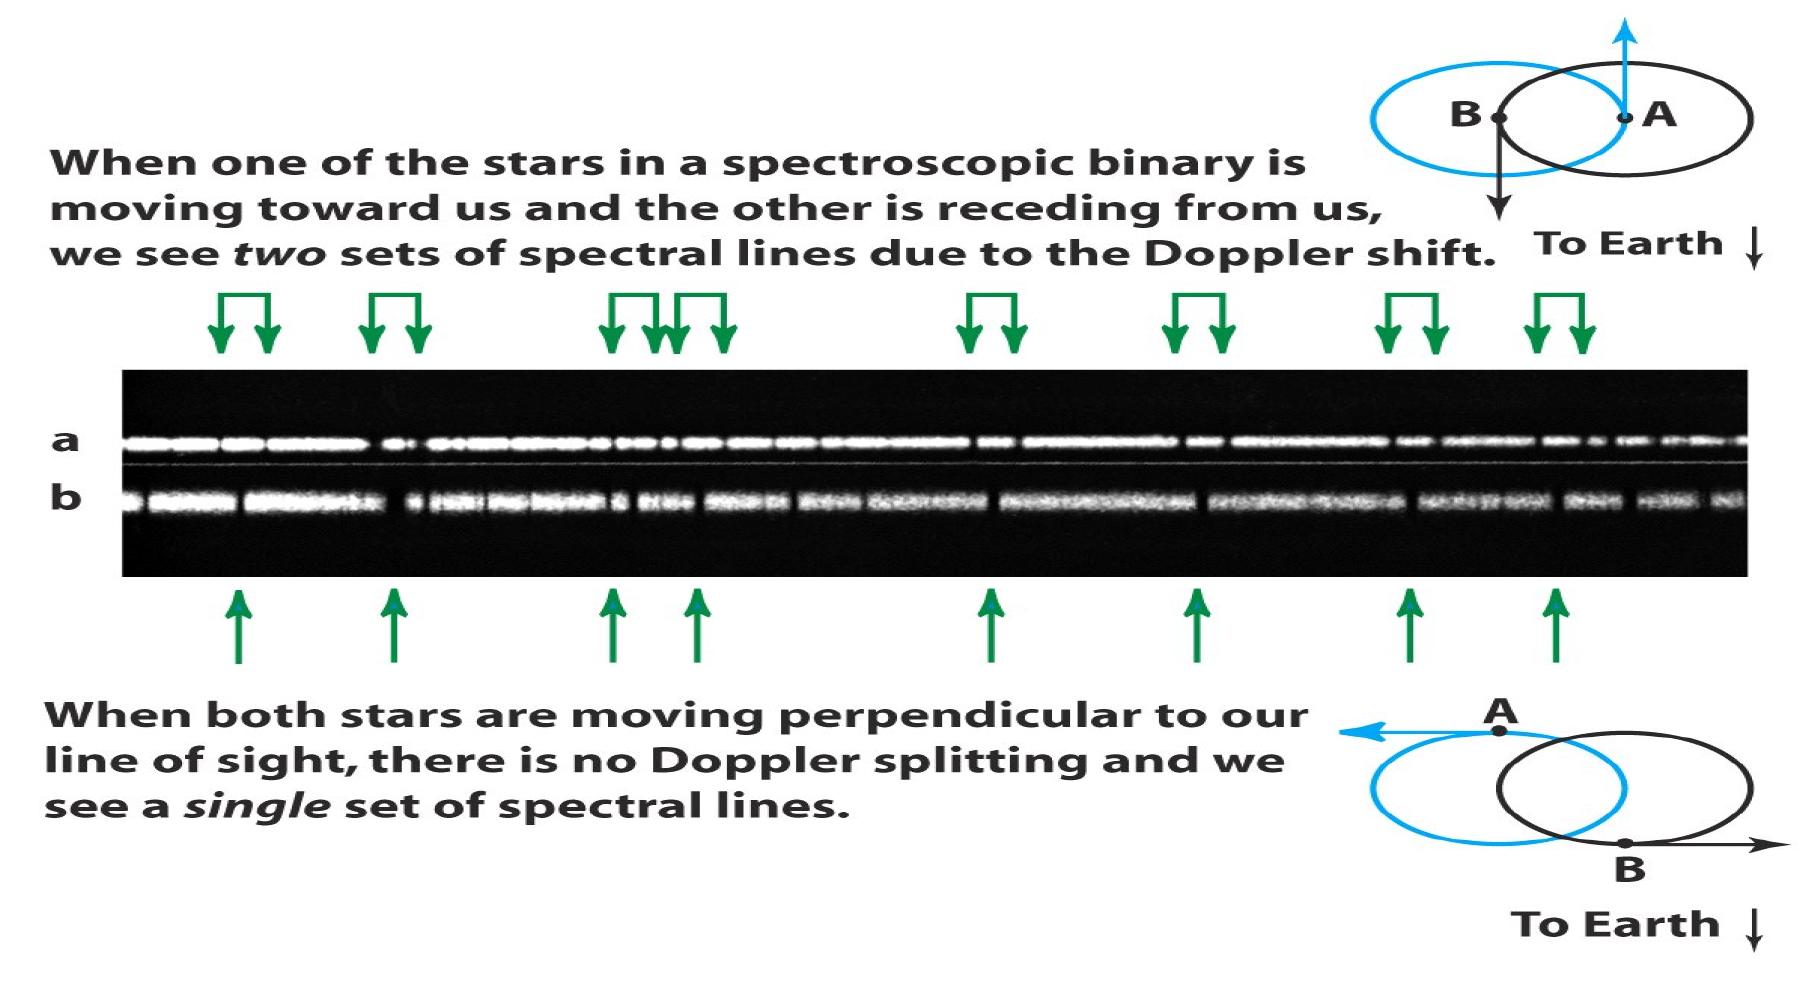
\includegraphics[scale=0.4]{Figures/spectroscopic_binary.png}
            \caption{Φασματοσκοπικά διπλό σύστημα αστέρων.}
            \label{fig:spectroscopic_binary}
        \end{figure}
    Από το φάσμα που παίρνουμε, βλέπουμε ότι περιέχει γραμμές που ανήκουν σε δύο αστέρες (αν οι λαμπρότητες των μελών είναι συγκρίσιμες) ή μόνο σε έναν αστέρα (αν η λαμπρότητα του ενός είναι πολύ μεγαλύτερη από του άλλου). Κάθε φασματική γραμμή ``ταλαντώνεται'' περιοδικά γύρω από ένα μέσο μήκος κύματος. Προφανώς οι φασματικές γραμμές μετατοπίζονται προς το ερυθρό όταν ο αντίστοιχος αστέρας βρίσκεται στο τμήμα της τροχιάς που απομακρύνεται από τη Γη, και προς το κυανό όταν βρίσκεται στο τμήμα της τροχιάς που προσεγγίζει τη Γη (σχήμα \ref{fig:spectroscopic_binary}). Επειδή οι 2 αστέρες βρίσκονται πάντα σε αντιδιαμετρική θέση ως προς το ΚΜ, όταν οι φασματικές γραμμές του ενός αστέρα είναι μετατοπισμένες προς το ερυθρό, οι φασματικές γραμμές του άλλου είναι μετατοπισμένες προς το κυανό και αντίστροφρα. Οι περισσότεροι γνωστοί διπλοί αστέρες είναι φασματοσκοπικά διπλοί χωρίς αυτό να σημαίνει ότι δεν μπορούν να ανήκουν ταυτόχρονα και σε κάποια άλλη κατηγορία.
        
    Από τον χρόνο που χρειάζεται για να έχουμε δύο διαδοχικές ταυτήσεις των φασματικών γραμμών, μπορούμε να βρούμε την \textit{περίοδο} του συστήματος. Επίσης, ξέρουμε ότι η μετατόπιση από τη θέση ισορροπίας (της φασματικής γραμμής) εξαρτάται από τη συνιστώσα της \textit{ταχύτητας κατά μήκος της γραμμής παρατήρησης} (line of sight). Δεν έχουμε και τις 3 συνιστώσες για το διάνυσμα της ταχύτητας. Μέσω αυτής της συνιστώσας της ταχύτητας μπορούμε να βρούμε και την απόσταση των δύο σωμάτων μεταξύ τους (ανάλογα με το πως αλλάζει το πλάτος της ταχύτητας).
        
    \underline{Σημείωση}: Τα μήκη κύματος στα οποία εμφανίζονται οι μετατοπισμένες γραμμές απορρόφησης δεν αντιστοιχούν σε κανένα χημικό στοιχείο που μπορεί να δώσει μετάπτωση από μία ενεργειακή στιβάδα σε κάποια άλλη και να παράξει αυτά τα μήκη κύματος.
        
    Μέσω της μελέτης των φασματοσκοπικά διπλών αστέρων \textit{δεν} είναι δυνατόν να υπολογισθεί η μάζα των αστέρων του συστήματος, παρά μόνο ο λόγος των μαζών τους και το γινόμενο της κάθε μάζας επί την άγνωστη ποσότητα $\sin^3 i$, όπου $i$ είναι η γωνία κλίσης του επιπέδου της τροχιάς του διπλού συστήματος (σχήμα \ref{fig:inclination_angle}).
        \begin{figure}[h]
            \centering
            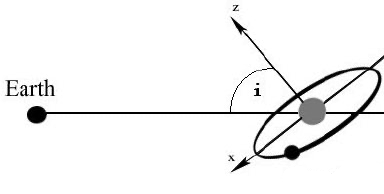
\includegraphics[scale=0.6]{Figures/inclination.jpg}
            \caption{Η γωνία κλίσης $i$, του επιπέδου της τροχιάς ενός διπλού συστήματος αστέρων.}
            \label{fig:inclination_angle}
        \end{figure}
        
    \item \textbf{Εκλειπτικά διπλοί αστέρες (ecliptic binaries)}\\
    Όταν το επίπεδο της τροχιάς των δύο αστέρων είναι σχεδόν παράλληλο με τη διεύθυνση παρατήρησης, δηλαδή η γωνία κλίσης $i \simeq 90^{\circ}$, και η απόσταση μεταξύ των μελών του συστήματος είναι πολύ μικρή, τότε κατά την περιφορά τους γύρω από το ΚΜ, τα 2 μέλη διέρχονται διαδοχικά το ένα μπροστά από το άλλο έτσι ώστε το ένα να καλύπτει τμήμα (ή και το σύνολο) του φαινόμενου δίσκου του άλλου, προκαλώντας μερικές ή όλικές εκλείψεις.
    Η ύπαρξη του ζεύγους συνεπάγεται από τις περιοδικές μεταβολές (αυξομειώσεις) της φαινόμενης λαμπρότητας του --φαινομενικά απλού-- αστέρα, η οποία μειώνεται κατά τη διάρκεια της έκλειψης.
    
    Κατά τη διάρκεια μίας περιφοράς συμβαίνουν δύο εκλείψεις, ανάλογα με το ποιό αστέρι βρίσκεται μπροστά από το άλλο και ως εκ τούτου παρουσιάζονται δύο ελάχιστα λαμπρότητας (σχήμα \ref{fig:eclipsing_binary}). Τα δύο αυτά ελάχιστα διαφέρουν γενικά ως προς το πλάτος και το βάθος, ανάλογα με τη λαμπρότητα των μελών του συστήματος.
        \begin{figure}[h]
            \centering
            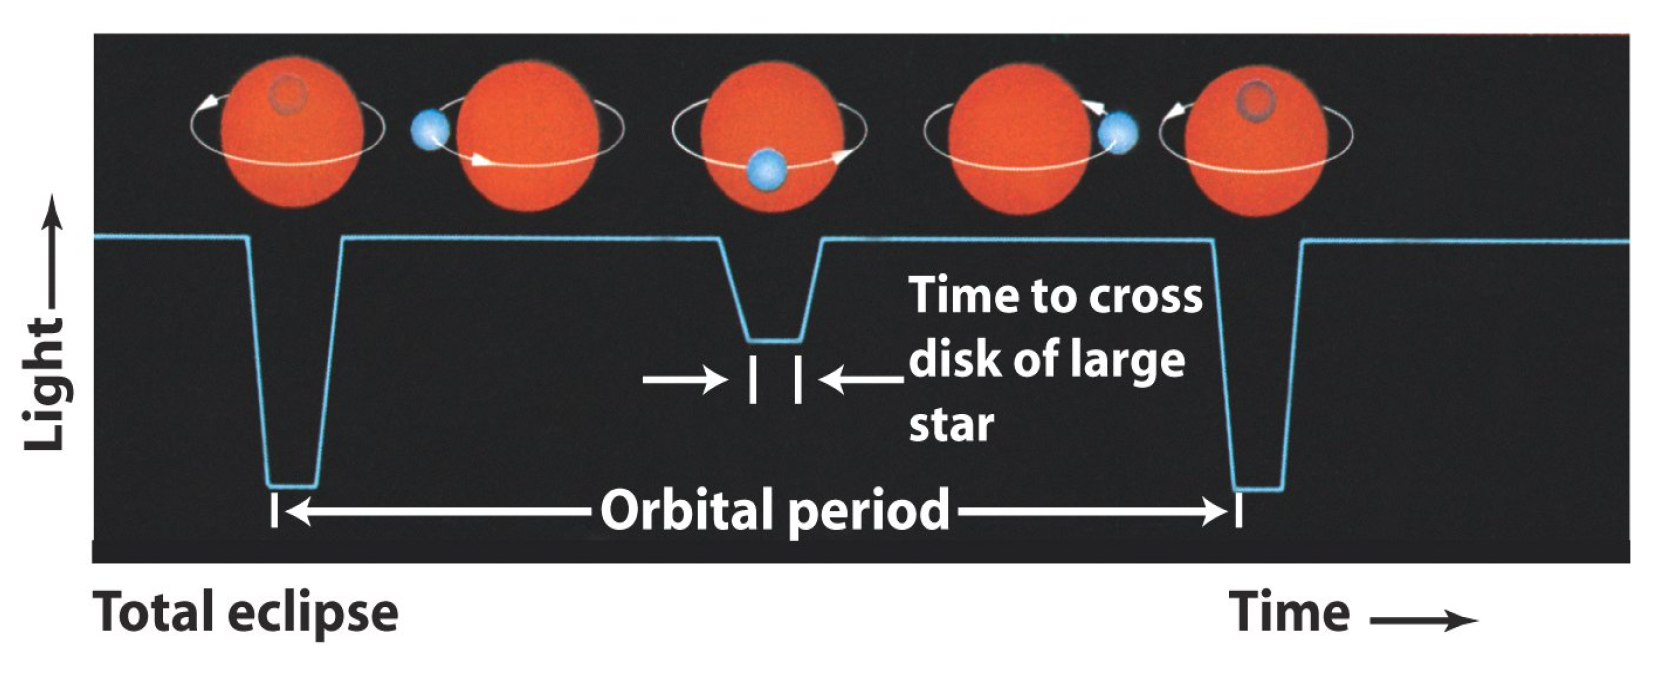
\includegraphics[scale=0.4]{Figures/eclipsing_binary.png}
            \caption{Καμπύλη φωτός για ένα εκλειπτικά διπλό σύστημα αστέρων. Όταν ο αμυδρότερος αστέρας καλύπτει τον λαμπρότερο έχουμε το \textit{πρωτεύον ελάχιστο}. Στην αντίθετη περίπτωση έχουμε το \textit{δευτερεύων ελάχιστο}.}
            \label{fig:eclipsing_binary}
        \end{figure}
        
    Και σε αυτή την περίπτωση δεν μπορούμε να υπολογίσουμε τη μάζα κανενός από τους αστέρες του συστήματος. Από την καμπύλη φωτός όμως (σχήμα \ref{fig:eclipsing_binary}) μπορούμε να υπολογίσουμε την κλίση της τροχιάς, τις ακτίνες των μελών του ζεύγους και τον λόγο των φωτεινοτήτων των δύο αστέρων. Αν επιπροσθέτως τα δύο αστέρια ανήκουν στην κύρια ακολουθία μπορούμε να υπολογίσουμε και τον λόγο των μαζών από τη σχέση μάζας-φωτεινότητας.
    
    \item \textbf{Αστρομετρικά διπλοί αστέρες (astrometric binaries)}\\
    Στη κατηγορία αυτή κατατάσσονται τα μη-οπτικώς διπλά συστήματα αστεριών, των οποίων ο αμυδρός συνοδός αστέρας εντοπίζεται μόνο μέσω των δυναμικών επιδράσεων του πάνω στην τροχιά του πρωτεύοντος αστέρα. Ουσιαστικά παρατηρούμε μόνο ένα άστρο, επειδή όμως η κίνηση στην τροχιά του παρουσιάζει παλινδρομήσεις, συμπεραίνουμε ότι υπάρχει αμυδρός συνοδός.
    
    \item \textbf{Φασματικά διπλοί αστέρες (spectral binaries)}\\
    Αν οι τυπικές ταχύτητες περιφοράς των μελών ενός διπλού συστήματος ή/και η γωνία κλίσης $i$ είναι πολύ μικρή, τότε δεν είναι δυνατόν να ανιχνευθεί η μετατόπιση Doppler των φασματικών γραμμών και επομένως το σύστημα δεν αναγνωρίζεται ως φασματοσκοπικά διπλός αστέρας. Παρόλα αυτά, αν τα δύο μέλη έχουν σημαντικά διαφορετικά φάσματα (ανήκουν δηλαδή σε διαφορετικούς φασματικούς τύπους) και συγκρίσιμες λαμπρότητες (έτσι ώστε και τα δύο φάσματα να είναι ορατά), τότε το σύστημα μπορεί να αναγνωριστεί ως φασματικά διπλός αστέρας.
    
    Είναι φανερό ότι οι φασματικά διπλοί αστέρες διαφέρουν από τους φασματοσκοπικά διπλούς στο ότι στους πρώτους δεν παρατηρείται μετατόπιση Doppler των γραμμών. Κανένα στοιχείο δεν μπορεί να βρεθεί για τους φασματικά διπλούς αστέρες αφού δεν παρατηρούμε σ' αυτούς κανένα φαινόμενο που να εμφανίζει χρονική μεταβολή.
\end{enumerate}

\subsection{Βασικοί υπολογισμοί}

\subsubsection{Υπολογισμός στοιχείων τροχιάς}
Μετατρέποντας τη \textit{σχετική φαινόμενη τροχιά} σε \textit{σχετική πραγματική τροχιά}, υπολογίζουμε τις εξής ποσότητες:
\begin{eqnarray*}
    \epsilon_{\pi} &=& \ \text{εκκεντρότητα} \\
    \alpha_{\pi} &=& \ \text{μεγάλος γωνιώδης ημιάξονας σε AU} \\
    i &=& \ \text{γωνία κλίσης}
\end{eqnarray*}

Αν γνωρίζουμε την παράλλαξη $p$, τότε υπολογίζουμε τον μεγάλο ημιάξονα $\alpha$ σε AU
\begin{equation}
    \alpha = \frac{\alpha_{\pi}}{p}
\end{equation}

\subsubsection{Υπολογισμός αθροίσματος μαζών}
Από τον 3ο νόμο του Kepler (σχέση \eqref{eq:Kepler_third_law}) έχουμε ότι 
$$M_1 + M_2 \simeq \frac{\alpha ^3}{P^2}$$ όπου $\alpha$ είναι ο μεγάλος ημιάξονας σε AU και $P$ η περίοδος του συστήματος.


\subsubsection{Υπολογισμός μαζών $M_1. M_2$}
Για φωτεινά διπλά συστήματα με σχετικά μεγάλη γωνιώδη απόσταση $\alpha_{\pi}$, μπορούμε να υπολογίσουμε και την \textit{απόλυτη φαινόμενη τροχιά} για καθένα από τα δύο μέλη. Άρα υπολογίζουμε δύο ημιάξονες $\alpha_1, \alpha_2$.

Από τον ορισμό του ΚΜ του συστήματος (σχέση \eqref{eq:center_mass}) και σε συνδυασμό με τον υπολογισμό του αθροίσματος $M_1 + M_2$ προκύπτουν οι μάζες $M_1, M_2$ για κάθε αστέρα.

\subsubsection{Δυναμικές παραλλάξεις}
 Από τις σχέσεις:
 \begin{eqnarray*}
    M_1 + M_2 &=& \frac{\alpha^3}{P^2} \\\\
    \alpha &=& \frac{\alpha_{\pi}}{p} 
 \end{eqnarray*}
 προκύπτει ότι:
 \begin{equation}
     \alpha_{\pi} = p \left[ (M_1 + M_2)P^2 \right]^{1/3}
 \end{equation}
 
 Αν οι δύο αστέρες ανήκουν στην κύρια ακολουθία, τότε για τον καθένα ισχύει ο νόμος μάζας-φωτεινότητας $L = f(M)$. Οπότε λύνουμε επαναληπτικά το σύστημα:
 
 \begin{eqnarray*}
    p &=& \alpha_{\pi} \left[ (M_1 + M_2)P^2 \right]^{-1/3} \\\\
    L_1 &=& f(M_1) \\\\
    L_2 &=& = f(M_2)
 \end{eqnarray*}
 για $\pi, M_1, M_2$ ξεκινώντας από κάποια εκτίμηση για το $M_1 + M_2$.  




\subsection{Στενά διπλά συστήματα \& απώλεια μάζας}
Κατά τη διάρκεια της ζωής τους, τα αστέρια χάνουν μάζα η οποία εμπλουτίζει τον μεσοαστρικό χώρο μέσω δύο διακασιών:
\begin{enumerate}[label=(\alph*)]
    \item \textbf{Συνεχώς}, μέσω των αστρικών ανέμων. Η μάζα που μπορεί να χαθεί με αυτόν τον τρόπο εξαρτάται από τη μάζα του αστέρα καθώς και το στάδιο της εξέλιξής του ($\dot{M}_{\text{Giant}} > \dot{M}_{MS}$).
    \item \textbf{Εκρηκτικώς}, μέσω καινοφανών και υπερκαινοφανών εκρήξεων.
\end{enumerate}

{\color{red} \hrule}
Στην περίπτωση ενός στενού διπλού συστήματος, οι αλληλεπιδράσεις μεταξύ των μελών μπορεί να οδηγήσει σε μεταφορά μάζας από το ένα αστέρι στο άλλο, επηρεάζοντας με αυτόν τον τρόπο την δομή, την μάζα, την γωνιακή στροφορμή καθώς και την τελική κατάσταση των αστέρων του συστήματος.\\
{\color{red} \hrule}

Όταν έχουμε ένα διπλό σύστημα, το πρόβλημα των πολλών σωμάτων (n-body problem) εκφυλίζεται στο ``περιορισμένο κυκλικό πρόβλημα των τριών σωμάτων'' (circular restricted three-body problem), με το ενεργό (effective) δυναμικό να δίνεται από τη σχέση:
\begin{equation}
    \label{eq:effective_potential}
    \Phi = - G \left( \frac{M_1}{r_1} + \frac{M_2}{r_2} \right) - \frac{1}{2} \Omega^2 r_3^2
\end{equation}
όπου  $r_1, r_2$ είναι οι αποστάσεις από το κέντρο των αστέρων $M_1, M_2$ αντίστοιχα, $\Omega$ είναι η τροχιακή γωνιακή ταχύτητα και $r_3$ είναι η απόσταση του άξονα περιστροφής τους συστήματος.

Η ποσότητα $\displaystyle V_g = - G \left( \frac{M_1}{r_1} + \frac{M_2}{r_2} \right)$ είναι ουσιαστικά το βαρυτικό δυναμικό ενώ το $\displaystyle V_F = - \frac{1}{2} \Omega^2 r_3^2$ περιγράφει το ``δυναμικό'' της φυγόκεντρου δύναμης. 

Αν απαιτήσουμε η συνολική δύναμη που ασκείται σε ένα δοκιμαστικό σωματίδιο, $m$, να είναι μηδέν: $$\boldsymbol{F_t} = - \nabla \Phi = 0$$
τότε η εξίσωση \eqref{eq:effective_potential} δίνει πέντε λύσεις όπου η βαρυτική δύναμη εξισορροπεί την φυγόκεντρο δύναμη που προκαλείται από τη σχετική κίνηση των δύο αστέρων του ενός γύρω από τον άλλον. Τα σημεία για τα οποία ισχύει αυτό, δηλαδή τα σημεία τα οποία έχουν μηδενική στιγμιαία ταχύτητα ονομάζονται \textit{σημεία Lagrange}, ($L_n, n = 1, \dots, 5$). Άρα αν το δοκιμαστικό σωματίδιο τοποθετούνταν σε κάποιο από αυτά τα σημεία, θα διατηρούσε τη θέση του σε σχέση ως προς τα δύο αστέρια.

Το σύνολο των σημείων μηδενικής ταχύτητας συγκροτεί μία ομάδα κλειστών επιφανειών, τις οποίες ονομάζουμε \textit{επιφάνειες μηδενικής ταχύτητας} (zero velocity surfaces) και περνούν από τα σημεία Lagrange. Η τομή μιας τέτοιας επιφάνειας μηδενικής ταχύτητας (ή ισοδυναμική επιφάνεια καθώς περιλαμβάνει όλα τα σημεία του συστήματος που μοιράζονται την ίδια τιμή του δυναμικού $\Phi$) με κάποιο συγκεκριμένο επίπεδο ονομάζεται \textit{καμπύλη μηδενικής ταχύτητας} (zero velocity curve). Συνήθως σαν επίπεδο τομής επιλέγεται το επίπεδο της σχετικής τροχιάς των δύο αστέρων του συστήματος (σχήμα \ref{fig:eq_sur}).
\\
{\color{red} \hrule}
Οι επιφάνειες μηδενικής ταχύτητας είναι σημαντικές γιατί ορίζουν τα όρια (boundaries) των περιοχών από τις οποίες το δοκιμαστικό σωματίδιο είναι δυναμικά αποκλεισμένο. Με άλλα λόγια, κάθε αστέρας ελέγχει βαρυτικά μόνο έναν περιορισμένο χώρο που καθορίζεται από μία ισοδυναμική επιφάνεια.\\
{\color{red} \hrule}

\begin{figure}[h]
   \centering
\begin{subfigure}[h]{0.45\textwidth}
	\centering
   	 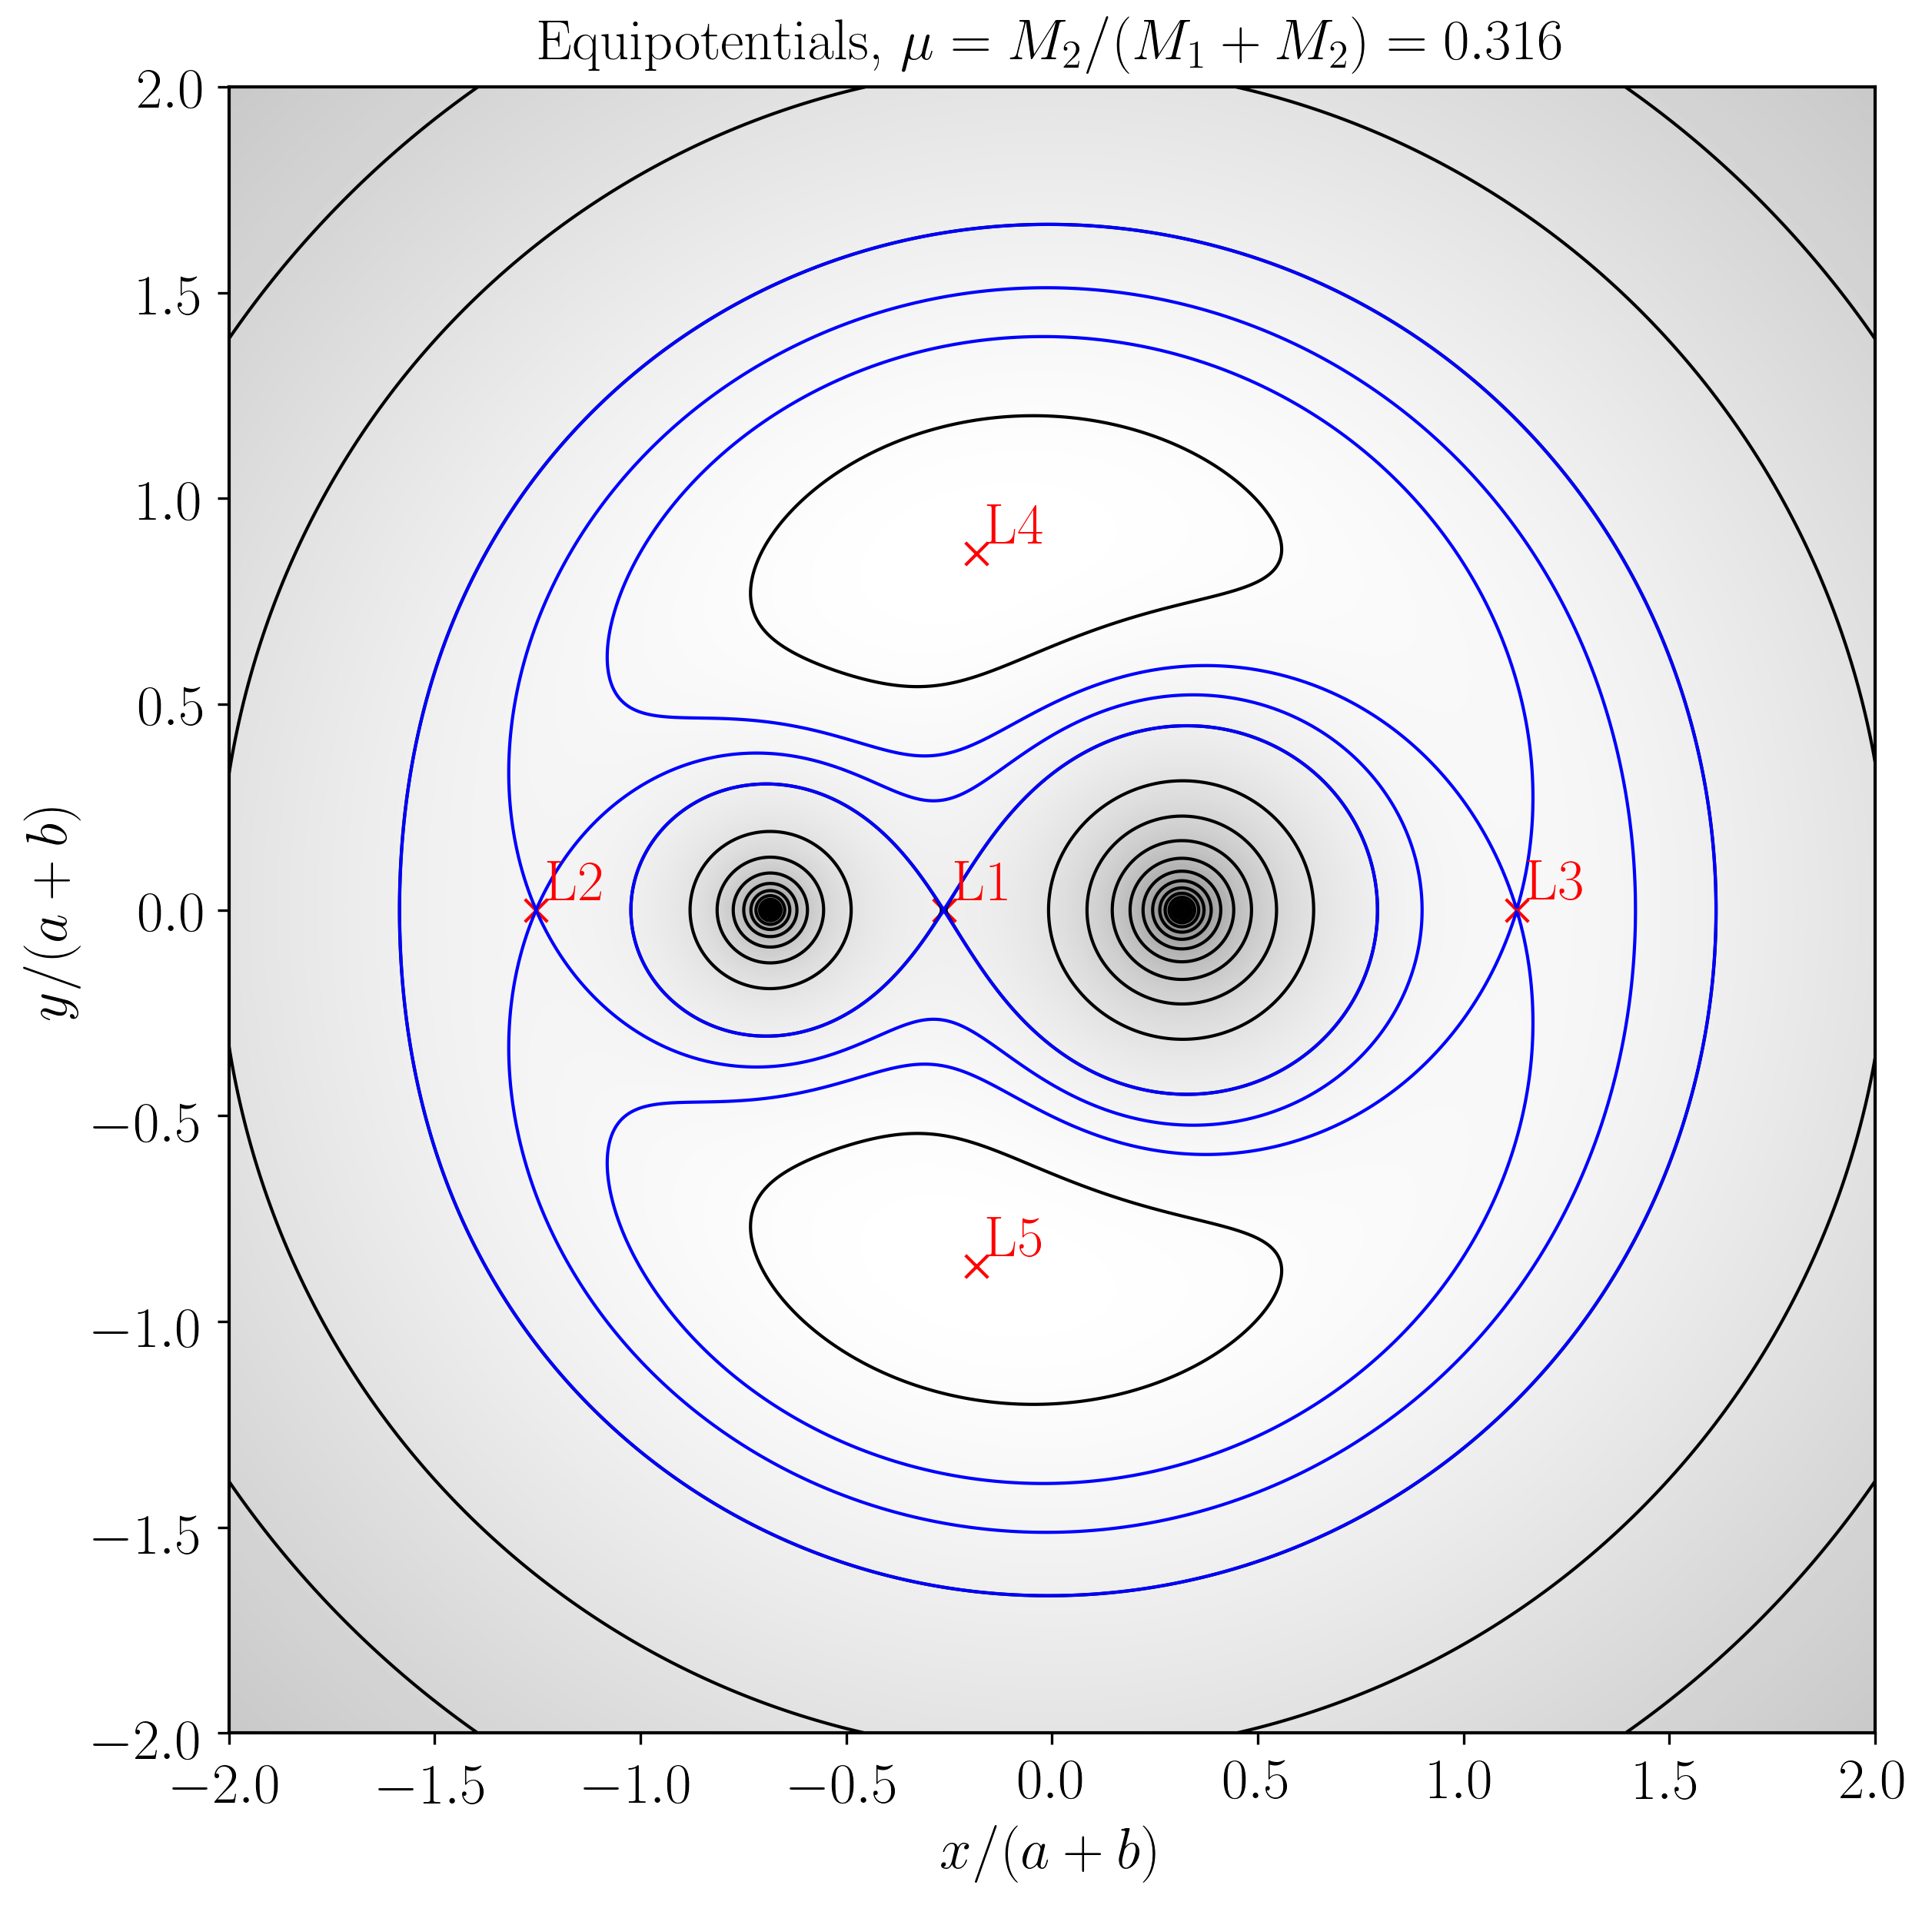
\includegraphics[width = \linewidth]{Figures/equipotentials_mu_0_316.png} 
\end{subfigure}
\begin{subfigure}[h]{0.535\textwidth}
	\centering
	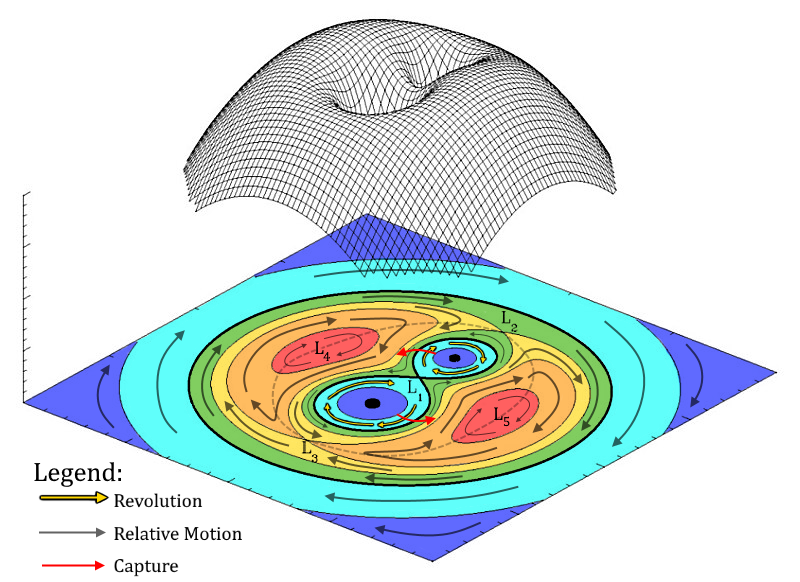
\includegraphics[width = \linewidth]{Figures/RochePotential_-_Colorized.png} 
    \end{subfigure}
    \caption{\textbf{Αριστερά}: Ισοδυναμικές γραμμές πάνω στο τροχιακό επίπεδο ενός περιστρεφόμενου διπλού συστήματος, με ανηγμένη μάζα $\mu = 0.316$ (reduced mass ratio). Σε αυτή τη διάταξη, $M_1$ είναι το αστέρι με τη μεγαλύτερη μάζα και βρίσκεται στη θέση $x = +a$, ενώ το $M_2$ είναι το αστέρι με τη μικρότερη μάζα και βρίσκεται στη θέση $x = -b$. Η εσωτερική ισοδυναμική επιφάνεια που περνάει από το σημείο Lagrange $L_1$, ορίζει τον λοβό Roche, που έχει σχήμα σταγόνας, για τον κάθε αστέρα. \textbf{Δεξιά}: 3D αναπαράσταση ισοδυναμικών επιφανειών.}
    \label{fig:eq_sur}
\end{figure}

Στο σχήμα \ref{fig:eq_sur} κάθε καμπύλη μηδενικής ταχύτητας έχει παρουσιαστεί με διαφορετικό χρώμα. Από τα πέντε σημεία Lagrange, το $L_1$ παίζει σημαντικό ρόλο στην εξέλιξη των διπλών συστημάτων καθώς η ισοδυναμική επιφάνεια που περνάει από αυτό ορίζει τους (ανεξάρτητους μεταξύ τους) \textit{λοβούς Roche} και κάθε ένας από αυτούς περιβάλλει έναν αστέρα του συστήματος.

Η επιφάνεια μηδενικής ταχύτητας που περνάει από το $L_1$ έχει ένα ιδιαίτερο χαρακτηριστικό: όλες οι επιφάνειες μηδενικής ταχύτητας που περιβάλλουν ένα μόνο σώμα, βρίσκονται μέσα στον αντίστοιχο λοβό Roche, ενώ όλες οι επιφάνειες μηδενικής ταχύτητας που βρίσκονται έξω από τους λοβούς Roche περιβάλλουν και τα δύο σώματα. Έτσι, ένα δοκιμαστικό σωματίδιο που βρίσκεται μέσα στο λοβό Roche ενός μέλους του διπλού συστήματος ``ανήκει'' βαρυτικά σε αυτόν τον αστέρα. Αντίθετα, ένα σωματίδιο που βρίσκεται έξω και από τους δύο λοβούς Roche ``ανήκει'' βαρυτικά και στους δύο αστέρες, αφού κινείται σε τροχιά που είναι δυνατόν να περιβάλλει και τους δύο. Οι τροχιές αυτές δεν είναι κωνικές τομές (κύκλοι, ελλείψεις, παραβολές, υπερβολές ή ευθείες).

Με βάση το λόγο της ακτίνας του κάθε αστέρα ως προς την ακτίνα του δικού του λοβού ($R_L$), τα διπλά συστήματα χωρίζονται στις εξής κατηγορίες:

\subsubsection{Αποχωρισμένα (detached binaries)}
Είναι ένα διπλό σύστημα στο οποίο ο κάθε ένας αστέρας βρίσκεται εξ' ολοκλήρου μέσα στον δικό του λοβό Roche και εξελίσσονται σχεδόν ανεξάρτητα ο ένας από τον άλλον. Ισχύει δηλαδή ότι $r_1 < R_{L,1}$ και $r_2 < R_{L,2}$ όπου $r_1, r_2$ οι ακτίνες των δύο αστέρων.

\subsubsection{Ημιαποχωρισμένα (semidetached binaries)}
Αυτά είναι τα συστήματα στα οποία μόνο ο ένας από τους δύο αστέρες ``γεμίζει'' τον λοβό Roche του (δηλαδή $r_1 < R_{L,1}$ και $r_2 \approx R_{L,2}$). Αυτό μπορεί να συμβεί σε μετεγενέστερα εξελικτικά στάδια στη διάρκεια ζωής ενός αστέρα, όταν μπει στη φάση των γιγάντων,
Έκεί, η ακτίνα του μεγαλώνει σε τόσο βαθμό όπου ο όγκος του αστέρα είναι συγκρίσιμος με  τον όγκο που ορίζει ο λοβός Roche του.

Σε αυτή την περίπτωση έχουμε εκροή μάζας από αυτόν τον αστέρα προς τον συνοδό του διαμέσου το εσωτερικού $L_1$ σημείο Lagrange. Η προσαύξηση του υλικού γίνεται με τον σχηματισμό ενός \textit{δίσκου επισυσσώρευσησ/προσαύξησης} και όχι με το να πέφτει απευθείας πάνω στον συνοδό αστέρα. Αυτό συμβαίνει διότο το υλικό που εκρύεται έχει την ίδια στροφορμή με τον αστέρα-δότη και εκτός αν υπάρχουν μη-συντηρητικές μηχανισμοί για να αφαιρέσουν ένα ποσό από τη στροφορμή του αερίου που εκρύεται, αυτό θα συνεχιστεί να περιφέρεται γύρω από τον συνοδό αστέρα. Για να καταφέρει να πέσει πάνω στον αστέρα, η ύλη πρέπει να χάσει στροφορμή από την εσωτερική τριβή (ιξώδες). Αυτή η εσωτερική τριβή του αερίου το αναγκάζει να θερμανθεί και να ακτινοβολεί (X-ray binary).

Η υπερχείλιση του αστέρα μέσα από τον λοβό του Roche οδηγεί σε σημαντική μείωση της μάζας του αστέρα και επηρεάζει τη μετέπειτα εξέλιξή του. Πέρα από αυτόν τον μηχανισμό όμως, μπορούμε να έχουμε μεταφορά μάζας με προσαύξηση από τον \textit{αστρικό άνεμο} του θερμότερου αστέρα προς τον ψυχρότερο. Παρόλα αυτά, η μεταφορά μάζας με αυτόν τον τρόπο δεν είναι το ίδιο αποδοτική όσο η υπερχείλιση του λοβού Roche.

\subsubsection{Εν επαφή (contact binary)}
Ένα διπλό σύστημα λέμε ότι είναι σε επαφή ότα και τα δύο αστέρια ``γεμίζουν'' τους λοβούς τους (δηλαδή $r_1 \approx R_{L,1}$ και $r_2 \approx R_{L,2}$). Σε αυτή την περίπτωση, το σύστημα μοιράζεται μία κοινή ατμόσφαιρα (common envelope, σχήμα \ref{fig:binary_cases}) η οποία μπορεί να εκδιωχθεί στερώντας έτσι από το σύστημα ένα σημαντικό μέρος της μάζας του.

\begin{figure}
    \centering
    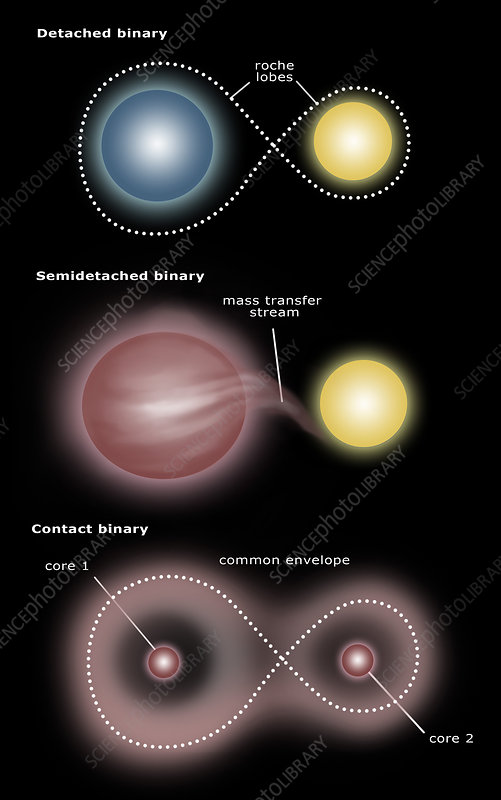
\includegraphics[scale=0.3]{Figures/binary_cases.jpeg}
    \caption{Κατηγορίες διπλών συστημάτων βάσει του ποσοστού πλήρωσης των λοβών Roche.}
    \label{fig:binary_cases}
\end{figure}

Σε αυτό το σημείονα διευκρινήσουμε ότι δεν υπάρχει αναλυτική έκφραση για το μέγεθος του λοβού Roche σε ένα διπλό σύστημα. Παρόλα αυτά έχει προταθεί μια αριθμητική προσέγγιση της ακτίνας του λοβού Roche μέσω της σχέσης:
$$\frac{R_L}{a} = \frac{0.49q^{2/3}}{0.6q^{2/3} + \ln (1 + q^{1/3})}$$
όπου $a$ είναι ο τροχιακός διαχωρισμός (orbital separation) του συστήματος και $\displaystyle q \equiv \frac{M_{\text{donor}}}{M_{\text{accretor}}}$ είναι ο λόγος των μαζών των μελών του συστήματος.
Αυτές είναι και οι δύο πιο σημαντικές παράμετροι για να ακολουθήσουμε την εξέλιξη του συστήματος.













\section{Μεταβλητοί αστέρες}
Μεταβλητοί αστέρες ονομάζονται οι αστέρες, των οποίων η λαμπρότητα μεταβάλλεται μέσα σε ένα χρονικό διάστημα σημαντικά μικρότερο από την ηλικία τους. Με τον (γενικά ασαφή) αυτό ορισμό αποφεύγει κανείς να χαρακτηρίσει μεταβλητούς όλους τους αστέρες, αφού, η λαμπρότητα ενός αστέρα μεταβάλλεται σημαντικά, και μάλιστα κατά πολλές τάξεις μεγέθους, στη διάρκεια της ζώης τους (π.χ. εγκατάσταση στην κύρια ακολουθία, άνοδος στον κλάδο των γιγάντων κτλ.)

Οι μεταβλητοί αστέρες κατατάσσονται σε κατηγορίες, ανάλογα με το φαινόμενο που προκαλεί τη μεταβολή της λαμπρότητά τους, την περιοδικότητα (ή την έλλειψη αυτής) της μεταβολής και το μέγεθός της. Καταρχάς, οι μεταβλητοί αστέρες μπορούν να χωριστούν σε γνήσιους μεταβλητούς και σε μη-γνήσιους. Στην τελευταία περίπτωση, η μεταβολή της λαμπρότητας του αστέρα δεν οφείλεται σε κάποιον ενδογενή φυσικό μηχανισμό αλλά σε κάποιον εξωτερικό παράγοντα που επηρεάζει φαινομενικά την λαμπρότητα. 

Η απλούστερη περίπτωση ενός τέτοιου μη-γνήσιου μεταβλήτού αστέρα είναι εκείνη, κατά την οποία ο αστέρας είναι στην πραγματικότητα εκλειπτικά διπλός και η μεταβολή της λαμπρότητάς του οφείλεται στο γεγονός ότι, κατά την κίνησή τους, τα μέλη του διέρχονται διαδοχικά το ένα μπροστά από το άλλο, προκαλώντας εκλείψεις. Η διάρκεια των εκλείψεων, ο ρυθμός ελλάτωσης και αύξησης της λαμπρότητας του διπλού αστέρα κατά την αρχή και το τέλος των εκλείψεων, η αλλαγή του δείκτη χρώματος και η περίοδος του φαινομένου δίνουν πληροφορίες για την απόσταση μεταξύ των μελών, τη μάζα τους, τις διαστάσεις τους, το φασματικό τους τύπο κτλ.
Από την άλλη μεριά, οι γνήσιοι μεταβλητοί αστέρες χωρίζονται στις κατηγορίες που θα αναλύσουμε παρακάτω.

\subsection{Περιοδικοί}
\subsubsection{Κηφείδες}
Οι Κηφείδες αστέρες αποτελούν τη σημαντικότερη κατηγορία περιοδικών μεταβλητών αστέρων. Ονομάστηκαν έτσι καθώς ο πρώτος τέτοιος αστέρας που μελετήθηκε ήταν ο ``δ Κηφέως'' στον αστερισμό του Κηφέα. Οι Κηφείδες είναι γίγαντες αστέρες και παρουσιάζουν περιοδικές μεταβολές στη λαμπρότητά τους, με περίοδο από 1 εως 50 ημέρες. Κατά τη διάρκεια μιας περιόδου, εκτός από την λαμπρότητα του αστέρα, που μεταβάλλεται κατά $\Delta m \simeq 1$ μέγεθος, μεταβάλλονται επίσης και ο δείκτης χρώματός του, και επομένος ο φασματικός του τύπος (και άρα η επιφανειακή του θερμοκρασία). Συνέπεια του γεγονότος αυτού είναι ότι η θέση των αστέρων αυτών δεν μένει σταθερή στο διάγραμμα H-R αλλά μετατοπίζεται, εκτελώντας μία κλειστή τροχιά κατά τη διάρκεια μιας περιόδου.

Η μεταβολή της λαμπρότητας των Κηφείδων δεν οφείλεται μόνο στη μεταβολή της θερμοκρασίας των αστέρων αυτών, αλλά και σε μεταβολή της ακτίνας τους. Επομένως οι αστέρες αυτοί παρουσιάζουν \textbf{αναπάλσεις} (pulsations). Αυτές οι αναπάλσεις αφορούν τα εξωτερικά στρώματα του αστέρα και δεν οφείλονται σε μεταβολές του ρυθμού παραγωγής ενέργειας στον πυρήνα καθώς τέτοια φαινόμενα θα εξελίσσονταν στην θερμική χρονική κλίμακα που είναι της τάξης των δεκάδων χιλιάδων ετών. Γίνεται φανερό ότι οι Κηφείδες δεν είναι γεννημένοι μεταβλητοί, αλλά αποτελούν μία φάση στην εξέλιξη ορισμένων αστέρων, μετά την έξοδό τους από την κύρια ακολουθία.

Αποδεικνύεται ότι για τους Κηφείδες αστέρες ισχύει μία σχέση μεταξύ της περιόδου και της λαμπρότητας της μορφής
\begin{equation}
    \label{eq:cepheids_period_luminosity_relation}
    \log P = \alpha \log L + \beta 
\end{equation}
όπου $\alpha$ και $\beta$ είναι αριθμητικές σταθερές. Μερικές φορές αυτή η σχέση εκφράζεται και με όρους απόλυτου μεγέθους αντί λαμπρότητας. Σε συνδυασμό με τη παρατηρούμενη μεταβολή στο φαινόμενο μέγεθος των Κηφείδων, η σχέση \eqref{eq:cepheids_period_luminosity_relation} μπορεί να χρησιμοποιηθεί για την εκτίμηση της απόστασης μέσω του distance modulus. Μέχρι σήμερα, έχουν μετρηθεί οι αποστάσεις πολλών γαλαξιών που φιλοξενούν Κηφείδες αστέρες χρησιμοποιώντας αυτή την μέθοδο.

\subsubsection{RR Lyrae}
Οι αστέρες αυτοί είναι μεταβλητοί μικρής περιόδου, η μεταβολή της φωτεινότητας των οποίων οφείλεται επίσης σε σφαιρικα συμμετρικές (ακτινικές) αναπάλσεις. Είναι κιτρινόλευκοι γίγαντες αστέρες (οριζόντιος κλάδος στο διάγραμμα H-R) ενώ έχουν μάζα και περίοδο μικρότερες από αυτές των Κηφείδων ($M \simeq 0.5\,M_\odot$, $P \sim 0.2 - 1\,\text{ημέρα}$). Η λαμπρότητά τους είναι σχεδόν ανεξάρτητη της περιόδου αναπάλσεως και αντιστοιχεί σε απόλυτο μέγεθος $M_V = 0.6$. Οι αστέρες αυτοί, πάντως, είναι αμυδρότεροι από τους Κηφείδες, και έτσι δεν είναι ορατοί σε μεγάλες αποστάσεις. Επομένως είναι χρήσιμοι για μετρήσεις αποστάσεων μέσα στο Γαλαξία, αλλά όχι για μετρήσεις αποστάσεων άλλων γαλαξιών.

\subsubsection{Μακροπερίοδοι}
Κατά τα τελευταία στάδια της εξέλιξης αστέρων μικρών μάζας είναι δυνατόν να υπάρξει συντονισμός των εξωτερικών στρωμάτων ενός αστέρα με το ρυθμό παραγωγής ενέργειας κατά τις διαδοχικές εναλλαγές καύσης των φλοιών H και He. Ο αστέρας τότε παρατηρείται ως μακροπερίοδος \textbf{μεταβλητός τύπου Mira} (Mira variable) με περίοδο, $P$, μεταξύ 100 και 1000 ημερών και εύρος μεταβολής μεγέθους $\Delta m_V \simeq 2 - 6\,\text{μεγέθη}$.

Οι μεταβλητοί τύπου Mira είναι ψυχροί, ερυθροί γίγαντες αστέρες μικρής μάζας και φασματικού τύπου Μ. Στο φάσμα τους παρατηρούνται ιδιαίτερα ισχυρές μοριακές γραμμές απορρόφησης. Το μεγάλο εύρος της μεταβολής του μεγέθους αυτών των αστέρων μπορεί να εξηγηθεί από το γεγονός ότι ο συντελεστής απορρόφησης εξαρτάταται ισχυρά από τη θερμοκρασία.

\subsection{Μη-περιοδικοί}
\subsubsection{Ανώμαλοι - T Tauri}
Οι αστέρες αυτοί πήραν το όνομά τους από τον τυπικό εκπρόσωπό της κατηγορίας, το μεταβλητό αστέρα Τ στον αστερισμό του Ταύρου. Παρατηρησιακά οι αστέρες αυτοί χαρακτηρίζονται:
\begin{enumerate}
    \item από απότομες και βραχυχρόνιες αυξήσεις της φωτεινότητάς τους από λίγα δέκατα του μεγέθους μέχρι και 4 μεγέθη, τις οποίες διαδέχονται διαστήματα ηρεμίας που διαρκούν από λίγες ώρες μέχρι και 100 ημέρες,
    \item από φασματικές γραμμές λιθίου (οι οποίες δεν εμφανίζονται σε άλλους αστέρες καθώς το λίθιο εξαντλείται πολύ γρήγορα κατά την έναρξη των θερμοπυρηνικών αντιδράσεων στους αστέρες) και
    \item από ισχυρούς αστρικούς ανέμους.
\end{enumerate}

Από την ερυθρή χρώση του φωτός τους και από το φάσμα τους βρίσκουμε ότι περιβάλλονται από ένα νέφος αερίου και σκόνης και ότι η θέση τους στο διάγραμμα H-R είναι μεταξύ των ερυθρών γιγάντων και της κύριας ακολουθίας. Η παρουσία λιθίου και η θέση τους στο διάγραμμα H-R μας κάνουν να πιστεύουμε ότι οι αστέρες της κατηγορίας αυτής είναι αστέρες ``εν τη γενέσει τους'', δηλαδή αστέρες που βρίσκονται ακόμα στο τελευταίο στάδιο της βαρυτικής συστολής τους. Επομένως οι αστέρες αυτοί δεν έχουν φτάσει ακόμα στη κύρια ακολουθία.

\subsubsection{Ανώμαλοι - Αστέρες εκλάμψεων}
Οι αστέρες αυτοί είναι ψυχροί ερυθροί νάνοι της κύριας ακολουθίας, οι οποίοι παρουσιάζουν σε ακανόνιστα χρονικά διαστήματα απότομες και σύντομες αυξήσεις της φωτεινότητάς τους (κυρίως στα χρώματα B και U αλλά και στα ραδιοφωνικά μήκη κύματος) μέχρι και 6 μεγέθη, γνωστές ως \textbf{εκλάμψεις} (flares). Σήμερα πιστεύουμε ότι οι εκλάμψεις αυτών των αστέρων είναι της ίδιας φύσης με τις ηλιακές, οφείλονται δηλαδή σε απελευθέρωση μαγνητικής ενέργειας από επανασύνδεση μαγνητικών γραμμών (magnetic reconnection).

Η ενέργεια μιας τυπικής τέτοιας έκλαμψης είναι πολλές τάξεις μεγέθους μεγαλύτερη από την ενέργεια μιας τυπικής ηλιακής έκλαμψης. Η διαφορά αυτή αποδίδεται στο γεγονός ότι το μαγνητικό πεδίο των αστέρων εκλάμψεων είναι κατά πολύ ισχυρότερου του ηλιακού, επειδή η ζώνη μεταφοράς, στην ύπαρξη της οποίας οφείλεται το μαγνητικό πεδίο (σύμφωνα με τη θεωρία της μαγνητικής γεννήτριας του Parker), είναι πολύ μεγαλύτερη στους αστέρες εκλάμψεων. Πραγματικά, σήμερα πιστεύουμε ότι οι νάνοι της κύριας ακολουθίας φασματιών τύπων Μ3 - Μ9 δεν έχουν καθόλου ζώνη ακτινοβολίας, έτσι ώστε η ζώνη μεταφοράς καλύπτει όλο το εσωτερικό του αστέρα, εκτός από τον πυρήνα του.

\subsubsection{Ανώμαλοι - R Coronae Borealis}
Οι υπεργίγαντες αυτοί αστέρες φασματικού τύπου F χαρακτηρίζονται ως ``αντίστροφοι καινοφανείς'', διότι η φωτεινότητά τους ελλατώνεται ενίοτε κατά πολλά (έως και 9) μεγέθη μέσα σε πολύ μικρό χρονικό διάστημα (λίγες ημέρες), παραμένει χαμηλή για λίγο και στη συνέχεια επανέρχεται στην αρχική της τιμή. Γενικά το φάσμα τους είναι φτωχό σε γραμμές υδρογόνου και πλούσιο σε γραμμές άνθρακα. Η ασυνήθιστη αυτή χημική σύσταση οφείλεται είτε στη μεταφορά ύλης από τον πυρήνα προς τη φωτόσφαιρά τους (dredge up), είτε διότι κατά το στάδιο του γίγαντα έχασαν τους φλοιούς H και He που περιέβαλλαν τον πυρήνα.

Σύμφωνα με το πιο διαδεμένο πρότυπο, οι μεταβλητοί τύπου \textbf{R Coronae Borealis} (δηλαδή όμοιοι με τον μεταβλητό αστέρα R του αστερισμού του Βόρειου Στέφανου, R CBr) έχουν πολύ ισχυρούς αστρικούς ανέμους, με τους οποίους ο χώρος γύρω τους εμπλουτίζεται με ενώσεις άνθρακα. 'Οταν οι ενώσεις αυτές ψυχθούν, σχηματίζονται κόκκοι ανθρακούχου σκόνης οι οποίοι απορροφούν έντονα σε όλα τα μήκη κύματος. Σε αυτήν ακριβώς την απορρόφηση οφείλονται τα ελάχιστα της φωτεινότητας που παρατηρούμε. Η απορρόφηση όμως της ακτινοβολίας του αστέρα ανεβάζει τη θερμοκρασία των κόκκων της σκόνης, με αποτέλεσμα αυτοί να εξαχνωθούν και να επανέλθει ο αστέρας στην αρχική του φωτεινότητα.

\subsubsection{Καταστροφικοί - Γενικά στοιχεία}
Στους καταστροφικούς μεταβλητούς ανήκουν οι \textbf{καινοφανείς} (novae) και \textbf{υπερκαινοφανείς} (supernovae) αστέρες, κύριο χαρακτηριστικό των οποίων είναι η απότομη (σε διάστημα ωρών ως ημερών) και μεγάλη (πάνω από 4 και συχνά πάνω απο 10 μεγέθη) αύξηση της λαμπρότητάς τους. Η κατάταξη αυτών των αστέρων βασίζεται σε παρατηρησιακά κριτήρια και δεν αντανακλά απαραίτητα τους φυσικούς μηχανισμούς που προκαλούν τις τεράστιες αυτές αναλάμψεις. Αποτέλεσμα του γεγονότος αυτού είναι ότι αναλάμψεις που οφείλονται σε διαφορετικούς μηχανισμούς μπορεί να καταταγούν στην ίδια κατηγορία, ενώ αναλάμψεις που οφείλονται σε παρόμοιο μηχανισμό μπορεί να καταλήξουν σε διαφορετικές κατηγορίες.

Η απαίτηση που έχουμε από μια θεωρία για τη δημιουργία των καινοφανών και υπερκαινοφανών είναι να εξηγεί, τουλάχιστον, τη μορφή της καμπύλης φωτός (light curve) του αστέρα, δηλαδή να εξηγεί τον χρόνο ανόδου, τη μέγιστη λαμπρότητα, και το ρυθμό καθόδου, καθώς επίσης και το παρατηρούμενο φάσμα. Οι θεωρίες που έχουν προταθεί για την ερμηνεία των καινοφανών και υπερκαινοφανών μπορούν να καταταγούν σε δύο γενικές κατηγορίες:
\begin{enumerate}
    \item σε αυτές που αναφέρονται στην εξέλιξη \textbf{μεμονωμένων} αστέρων μεγάλης μάζας και
    \item σε αυτές που αναφέρονται στην εξέλιξη \textbf{διπλών συστημάτων} μέτριας μάζας.
\end{enumerate}
Σήμερα πιστεύουμε ότι οι υπερκαινοφανείς τύπου II ακολουθούν το πρώτο σενάριο, ενώ οι υπερκαινοφανείς τύπου I και οι καινοφανείς το δεύτερο σενάριο.

\begin{figure}
    \centering
    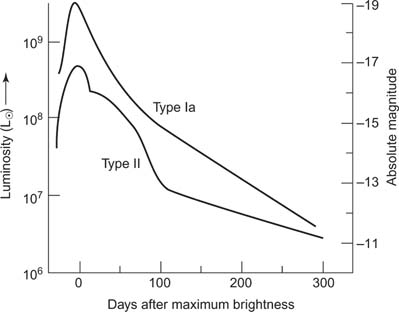
\includegraphics{Figures/sne_light_curves.jpeg}
    \caption{Καμπύλες φωτός υπερκαινοφανών αστέρων}
    \label{fig:sne_light_curves}
\end{figure}

\subsubsection{Καταστροφικοί - Καινοφανείς}
Σύμφωνα με το γενικά παραδεκτό σήμερα σενάριο, οι καινοφανείς αστέρες προέρχονται από την εξέλιξη διπλών συστημάτων. Σε ένα διπλό σύστημα με δύο αστέρες 1 και 2, που έχουν μάζες $M_1 > M_2$, ο αστέρας 1 εγκαταλείπει πρώτος την κύρια ακολουθία και αρχίζει να εξελίσσεται σε ερυθρό γίγαντα. Αν η απόσταση των δύο αστέρων ειναι αρκετά μικρή, τότε ο αστέρας 1 γεμίζει τον δικό του λοβό Roche, και μάζα από τα εξωτερικά του στρώματα μεταφέρεται στον αστέρα 2. 'Οταν τελειώσει αυτή η διαδικασία, τότε από τον αστέρα 1 δεν έχει απομείνει παρά μόνο ο πυρήνας του, ο οποίος τελικά καταλήγει (αν η μάζα του δεν υπερβαίνει το όριο Chandrasekhar) σε λευκό νάνο μάζας $M \sim 1\,M_\odot$. Παράλληλα ο αστέρας 2 έχει γίνει ήδη πολύ μεγαλύτερος (λόγω της προσαύξησης μάζας από τον αστέρα 1) και αρχίζει να εξελίσσεται με τη σειρά του σε ερυθρό γίγαντα. Κατά την εξέλιξη αυτή γεμίζει με τη σειρά του τον δικό του λοβό Roche, και αρχίζει πλέον η αντίστροφη μεταφορά μάζας από τον αστέρα 2 στον αστέρα 1 (λευκό νάνο).

'Οταν η μάζα της ύλης που συσσωρεύεται στη θερμή ατμόσφαιρα του λευκού νάνου ξεπεράσει κάποια κρίσιμη τιμή, τότε η πίεση και η θερμοκρασία στη βάση της ατμόσφαιράς του επιτρέπουν τη καύση του υδρογόνου σε ήλιο, αντίδραση που συμβαίνει σχεδόν ακαριαία. Η ενέργεια που εκλύεται από την έναρξη της θερμοπυρηνικής αυτής αντίδρασης απελευθερώνεται με τη μορφή μιας μεγάλης έκρηξης, που μπορεί να ανεβάσει τη λαμπρότητα του συστήματος κατά 10 μεγέθη, σε διάστημα μερικών ωρών.

Εφόσον η ροή ύλης από τον αστέρα 2 στον αστέρα 1 συνεχίζεται, μια τέτοια έκρηξη θα επαναλαμβάνεται κάθε φορά που η συσσωρευμένη μάζα ξεπερνά την κρίσιμη τιμή. Αν ο ρυθμός μεταφοράς είναι μεγάλος, τότε το πρότυπο αυτό προβλέπει ότι η κρίσιμη τιμή της μάζας είναι μικρή, επειδή η ύλη δεν προλαβαίνει να ``απλωθεί'' σε μεγάλη έκταση. Στην περίπτωση αυτή οι εκρήξεις αυτές επαναλαμβάνονται σε σύντομα χρονικά διαστήματα, αλλά είναι μικρές. Αντίθετα, αν ο ρυθμός μεταφοράς είναι μικρός, τότε οι εκρήξεις απέχουν χρονικά πολύ μεταξύ τους, αλλά είναι μεγάλες.

Σύμφωνα με το παραπάνω σενάριο, όλοι οι καινοφανείς πρέπει να είναι α) διπλοί και β) επαναληπτικοί. Τα μέχρι τώρα παρατηρησιακά δεδομένα υποστηρίζουν ικανοποιητικά την παραπάνω θεωρία σχηματισμού των υπερκαινοφανών. Ας σημειωθεί όμως ότι υπάρχουν και θεωρίες για την προέλευση των υπερκαινοφανών εκρήξεων που βασίζονται στην εξέλιξη απλών (μεμονωμένων) αστέρων, και δεν αποκλείεται μερικοί από τους καινοφανείς που παρατηρούμε να οφείλεται σε τέτοιες περιπτώσεις.

\subsubsection{Καταστροφικοί - Υπερκαινοφανείς I}
Για τους υπερκαινοφανείς τύπου I δεν υπάρχει σήμερα μια θεωρία τόσο γενικά παραδεκτή, όσο για τους υπερκαινοφανείς τύπου II ή τους καινοφανείς. Το πιο δημοφιλές σενάριο είναι παρόμοιο με αυτό των καινοφανών. Υπάρχει δηλαδή ένα διπλό σύστημα, το ένα μέλος του οποίου είναι ένας λευκός νάνος άνθρακα-οξυγόνου. Μάζα μεταφέρεται από τον συνοδό αστέρα στον λευκό νάνο και, έτσι, η μάζα του τελευταίου συνεχώς αυξάνει χωρίς την παρουσία εκρηκτικών αναλάμψεων αυτή το φορά. 'Οταν η μάζα του λευκού νάνου πλησιάζει το όριο Chandrasekhar, προκαλειται ανάφλεξη του άνθρακα στο εσωτερικό του λευκού νάνου και η παραγόμενη ενέργεια  θερμαίνει και εκτινάσσει τα ανώτερα στρώματα του αστέρα στο διάστημα. Η έκρηξη αυτή που ονομάζεται υπερκαινοφανής τύπου I είναι τόσο σφοδρή ώστε διαλύει το σύστημα και δεν αφήνει πίσω κάποιο συμπαγές αστρικό αντικείμενο, όπως π.χ. έναν αστέρα νετρονίων.

Το γεγονός ότι η έκρηξη συμβαίνει πάντα κοντά στην ίδια τιμή μάζας (όριο Chandrasekhar) σημαίνει ότι η ενέργεια από μία τέτοια έκρηξη (συγκεκριμένα από υπερκαινοφανείς τύπου Ia) είναι γνωστή (της τάξης των $10^{51}\,\text{erg}$). Αυτό μας επιτρέπει να χρησιμοποιήσουμε αυτές τις εκρήξεις ως ``σταθερά κεριά'' (standard candles) των οποίων γνωρίζουμε την λαμπρότητα, και άρα μπορούμε να τα χρησιμοποιήσουμε ως δείκτες για την μέτρηση αποστάσεων.


\subsubsection{Καταστροφικοί - Υπερκαινοφανείς II}
Σύμφωνα με την επικρατούσα σήμερα άποψη, η κατάληξη ενός αστέρα μεγάλης μάζας ($M > 5\,M_\odot$) είναι ένας υπερκαινοφανής τύπου II. Για αστέρες με μάζα στο διάστημα $5 < M/M_\odot < 10$ ο μηχανισμός του φαινομένου οφείλεται στην \textbf{έκρηξη άνθρακα} (carbon detonation) η οποία είναι παρόμοια με την λάμψη ηλίου που έχουμε περιγράψει αλλά πολύ πιο βίαιη. Για αστέρες με μάζα $M > 10\,M_\odot$ ο μηχανισμός του φαινομένου οφείλεται στην καταστροφική κατάρρευση ενός αδρανούς πυρήνα σιδήρου.

'Ενας αστέρας που έχει εξαντλήσει όλα τα πυρηνικά του καύσιμα (έχει δηλαδή δημιουργήσει έναν πυρήνα από σίδηρο), αρχίζει να καταρρέει, αφού δεν υπάρχει εσωτερική πηγή πίεσης που να αντισταθμίζει το βάρος των υπερκείμενων στρωμάτων. Επειδή η μάζα του πυρήνα είναι μεγαλύτερη από το όριο Chandrasekhar, η κατάρρευση δεν μπορεί να σταματήσει με τη δημιουργία ενός λευκού νάνου, και έτσι η κατάρρευση συνεχίζεται προς κατάστάσεις που χαρακτηρίζονται από ολοένα και μεγαλύτερη πυκνότητα. Η αδιαβατική συμπίεση του πυρήνα, που οφείλεται στη συνεχιζόμενη κατάρρευση, προκαλεί αύξηση της θερμοκρασίας του, η οποία ευνοεί τις ενδόθερμες πυρηνικές αντιδράσεις. 'Ετσι ο σίδηρος φωτοδιασπάται από τα φωτόνια υψηλών ενεργειών σύμφωνα με την αντίδραση
$$\rm Fe^{56} + h\nu \longrightarrow \rm 13 He^4 + 4n$$
ενώ στη συνέχεια διασπάται και το παραγόμενο ήλιο
$$\rm He^4 + h\nu \longrightarrow \rm 2p + 2n$$
Οι αντιδράσεις αυτές απορροφούν ενέργεια, ανακόπτουν την αύξηση της θερμοκρασίας και της πίεσης του πυρήνα και επιταχύνουν την κατάρρευση. Στα τελευταία στάδια η κατάρρευση επιταχύνεται ακόμη περισσότερο από τις πυρηνικές αντιδράσεις σύλληψης ηλεκτρονίου
$$\rm p + e^{-} \longrightarrow \rm n + \nu_e$$

Τα νετρίνα που παράγονται από τις παραπάνω αντιδράσεις διαφεύγουν έξω από τον πυρήνα, λόγω της μικρής ενεργού διατομής της αλληλεπίδρασης των νετρίνων με την ύλη (αδιαφάνεια ύλης στα νετρίνα $\kappa \simeq 0$). Με τη διαφυγή τους μεταφέρουν μεγάλα ποσά ενέργειας εκτός του πυρήνα και έτσι μετριάζουν ακόμα περισσότερο την πιεση και τη θερμοκρασία του. Κάτω από αυτές τις συνθήκες, η δύναμη της βαρύτητας σε κάθε στρώμα του αστέρα είναι πολύ μεγαλύτερη από τη δύναμη της πίεσης και η κατάρρευση των διάφορων στρωμάτων του αστέρα μοιάζει με ελεύθερη πτώση, η οποία για τον πυρήνα διαρκεί μερικά δευτερόλεπτα. Φυσικά η κατάρρευση αυτή, κατά την οποία η δυναμική βαρυτική ενέργεια της ύλης του αστέρα μετατρέπεται σε κινητική ενέργεια, δεν μπορεί να συνεχισθεί επ' άπειρο. 'Οταν η πυκνότητα του αστρικού πυρήνα φτάσει τα όρια της πυρηνικής πυκνότητας ($\sim 10^{14}\,\text{g cm$^{-3}$}$), η αδιαφάνεια των νετρίνων αυξάνει απότομα (η μέση ελεύθερη διαδρομή τους μειώνεται), έτσι ώστε να μην μπορούν πλέον να διαφύγουν ελεύθερα, μεταφέροντας ενέργεια έξω από τον πυρήνα. Επειδή ο πυρήνας δεν μπορεί να ψυχθεί μέσω της διαφυγής νετρίνων, η θερμοκρασία του αρχίζει να αυξάνει αδιαβατικά, προκαλώντας την αλματώδη αύξηση της πίεσης του αερίου στον πυρήνα, αλλά κυρίως την σχεδόν εκρηκτική αύξηση της πίεσης της ακτινοβολίας. Στο σημείο αυτό υπάρχουν δύο ενδεχόμενα:
\begin{enumerate}
    \item Η αρχική μάζα του αστέρα να ήταν εξαιρετικά μεγάλη. Στην περίπτωση αυτή η δύναμη της βαρύτητας παραμένει πάντα μεγαλύτερη της δύναμης της πίεσης, με αποτέλεσμα ο αστέρας να υποστεί ολοκληρωτική βαρυτική κατάρρευση και να καταλήξει σε μια μελανή οπή.
    \item Η αρχική μάζα του αστέρα δεν ήταν τόσο μεγάλη ώστε να μιλάμε για ολοκληρωτική νίκη της βαρύτητας. Στην περίπτωση αυτή η αύξηση της πίεσης δεν είναι δυνατόν να συνεχίζεται επ' άπειρον: φτάνει κάποια στιγμή, που η δύναμη της πίεσης προς τα έξω υπερισχύει κατά πολύ της δύναμης της βαρύτητας οπότε τα εξωτερικά στρώματα του πυρήνα ``αναπηδούν'', όπως μια ελαστική σφαίρα που προσκρούει σε μια σκληρή επιφάνεια, και αρχίζουν να διαστέλλονται με υπερηχητική ταχύτητα. Κατά την διαστολή τους δημιουργούν ένα κρουστικό κύμα το οποίο θερμαίνει και παρασύρει προς τα έξω τα υπόλοιπα στρώματα του αστέρα, που συνέχιζαν να καταρρέουν, και τα εκτινάσσει στο διάστημα. Ταυτόχρονα, τα άφθονα νετρόνια που είχαν δημιουργηθεί από τη φωτοδιάσπαση του σιδήρου και του ηλίου απορροφούνται από πυρήνες μεσαίου ατομικού αριθμού και σχηματίζουν όλα τα χημικά στοιχεία βαρύτερα του σιδήρου, τα οποία δεν είναι δυνατόν να σχηματιστούν με εξώθερμες θερμοπυρηνικές αντιδράσεις. 'Ενας υπερκαινοφανής τύπου II έχει μόλις δημιουργηθεί. Το μόνο που είναι δυνατόν αν απομείνει από την τεράστια αυτή έκρηξη είναι το κεντρικό τμήμα του αστρικού πυρήνα, που πιστεύουμε ότι σταθεροποιείται στην κατάσταση ενός αστέρα νετρονίων.
\end{enumerate}
